\subsubsection{强最大值原理}\label{subsec:strong-maximum-principle}

Theorem~\ref{thm:weak-maximum-principle} 指出, $u$ 在边界上取得最大值. 然而, $u$ 可能在许多点取得最大值, 因而该定理并未排除其中一些点是内点的可能性. 强最大值原理指出, 除非 $u$ 为常数, 否则这种情况不可能发生. 为证明这一点, 需要以下引理, 它本身也很有意义.

\begin{figure}[H]
\centering
\includegraphics[page=114,pagebox=cropbox,trim=96.60bp 415.60bp 93.82bp 45.92bp,clip,width=.78\linewidth]{../input/source/An Introduction to Partial Differential Equations.pdf}
\caption{}\label{fig:boundary-point-interior-ball}
\end{figure}

\begin{Lemma}
\label{lem:elliptic-boundary-point}
假设 $\Omega$ 位于 $\partial\Omega$ 的一侧. 假设 $Lu\geq0$, 并设 $\bm{x}_0$ 为 $\partial\Omega$ 上的一点, 使对每个 $\bm{x}\in\Omega$ 都有 $u(\bm{x}_0)>u(\bm{x})$. 再假设在 $\bm{x}_0$ 的一个邻域内, $\partial\Omega$ 是 $C^2$ 曲面, 且 $u$ 在 $\bm{x}_0$ 处可微. 此外, 假设以下情形之一成立:
\begin{enumerate}
\item $c=0$,
\item $c\leq0$ 且 $u(\bm{x}_0)\geq0$, 或
\item $u(\bm{x}_0)=0$
\end{enumerate}
那么 $\partial u/\partial n(\bm{x}_0)>0$, 其中 $\partial u/\partial n$ 表示沿 $\partial\Omega$ 的外法向的方向导数.
\end{Lemma}

\begin{Proof}
由于假设了 $\partial\Omega$ 为 $C^2$ 的, 可以选取 (见 Problem~\ref{ex:interior-tangent-ball}) 球 $B_R(\bm{y})$, 使 $B_R(\bm{y})\subset\Omega$ 且 $\bm{x}_0\in\partial B_R(\bm{y})$. 这里 $R$ 和 $\bm{y}$ 表示球的半径与球心.

对 $0\leq r=|\bm{x}-\bm{y}|\leq R$, 定义
\begin{equation}\label{eq:boundary-point-exponential-barrier}
v(\bm{x})=\exp(-\alpha r^2)-\exp(-\alpha R^2).
\end{equation}
得到
\begin{equation}\label{eq:boundary-point-barrier-operator}
\begin{aligned}
Lv(\bm{x})&=\exp(-\alpha r^2)\bigl[4\alpha^2a_{ij}(x_i-y_i)(x_j-y_j)\\
&\qquad-2\alpha(a_{ii}+b_i(x_i-y_i))\bigr]+cv.
\end{aligned}
\end{equation}
现在令 $A=B_R(\bm{y})\cap B_{R'}(\bm{x}_0)$, 其中 $R'$ 取得很小. 当 $\alpha$ 足够大时, 在 $A$ 内有 $Lv>0$. 此外, 若将 $\epsilon>0$ 取得足够小, 则在 $\partial A\cap\partial B_{R'}(\bm{x}_0)$ 上有 $u-u(\bm{x}_0)+\epsilon v\leq0$, 在 $\partial A\cap\partial B_R(\bm{y})$ 上也成立, 因为那里 $v=0$. 因此得到, 在 $A$ 内 $L(u-u(\bm{x}_0)+\epsilon v)\geq-cu(\bm{x}_0)\geq0$, 且在 $\partial A$ 上 $u-u(\bm{x}_0)+\epsilon v\leq0$.

若 $c\leq0$, 则弱最大值原理 (Corollary~\ref{cor:weak-maximum-nonpositive-zero-order}) 表明, 在整个 $A$ 内 $u-u(\bm{x}_0)+\epsilon v\leq0$. 在 $\bm{x}_0$ 处取外法向导数, 得到
\begin{equation}\label{eq:boundary-point-positive-normal-derivative}
\dfrac{\partial u}{\partial n}(\bm{x}_0)\geq-\epsilon\dfrac{\partial v}{\partial n}(\bm{x}_0)=2\alpha\epsilon R\exp(-\alpha R^2)>0,
\end{equation}
由此得出引理.

若 $u(\bm{x}_0)=0$, 则由假设, $u$ 在 $\Omega$ 内为负. 现在令 $c^+(\bm{x})=\max(0,c(\bm{x}))$. 得到 $(L-c^+)u=Lu-c^+u\geq Lu\geq0$, 因此可以用 $L-c^+$ 代替 $L$, 应用上述论证.
\end{Proof}

\begin{Remark}
\label{rem:boundary-one-side-jordan}
由于假设了 $\Omega$ 连通, 可以证明, 若 $\Omega$ 有界且 $\partial\Omega$ 整体光滑, 则 $\Omega$ 位于 $\partial\Omega$ 的一侧. (这是 Jordan 曲线定理的多维推广.) 证明可参见例如~\cite{Mas}.
\end{Remark}

\begin{Remark}
\label{rem:boundary-point-semidefinite}
若矩阵 $a_{ij}$ 仅半正定, 且 $\bm{n}$ 不属于零空间, Lemma~\ref{lem:elliptic-boundary-point} 仍然成立.
\end{Remark}

作为 Lemma~\ref{lem:elliptic-boundary-point} 的推论, 得到以下强最大值原理.

\begin{Theorem}
\label{thm:strong-maximum-principle}
假设在 $\Omega$ (不一定有界) 内 $Lu\geq0$ ($Lu\leq0$), 并假设 $u$ 不为常数. 若 $c=0$, 则 $u$ 不在 $\Omega$ 内部达到最大值 (最小值). 若 $c\leq0$, 则 $u$ 不能在内部达到非负的最大值 (非正的最小值). 无论 $c$ 的符号如何, $u$ 都不能在内部的最大值 (最小值) 点处为零.
\end{Theorem}

\begin{Proof}
假设 $u$ 在某内点取得最大值 $M$, 令 $\Omega^-=\Omega\cap\{u<M\}$. 若 $\Omega^-$ 非空, 则 $\partial\Omega^-\cap\Omega$ 非空. 设 $\bm{y}$ 是 $\Omega^-$ 中一点, 它到 $\partial\Omega^-$ 的距离小于到 $\partial\Omega$ 的距离, 并设 $B$ 为以 $\bm{y}$ 为球心且包含于 $\Omega^-$ 内的最大球. 取 $\bm{x}_0$ 为 $\partial B\cap\partial\Omega^-$ 上一点. 那么可以对 $B$ 应用前一个引理. 得到 $\nabla u$ 在 $\bm{x}_0$ 处非零, 与 $u$ 在那里取得最大值的假设矛盾.
\end{Proof}
